\documentclass[12pt,a4paper]{article}
\usepackage[utf8]{inputenc}
\usepackage{amsmath}
\usepackage{amsfonts}
\usepackage{amssymb}
\usepackage{graphicx}
\usepackage{subcaption}
\usepackage{float}
\usepackage{multirow}
\usepackage{rotating}
\usepackage{tikz}
\usepackage{pgfplots}
\usepackage[bottom]{footmisc}

\author{Team Gamma \\ {\small Ajda Frankovič, Martin Preradović, Niki Bizjak}}
\title{Final report}
\date{}
\begin{document}
	
	\maketitle
	
	\section{Introduction}
	% kaj je bil task
	% shema stanj robota
	
	\section{Methods} \label{methods}
	In this section, the algorithms and methods we have used in our system are presented.

	% Dodaj nek dictionary pojmov
	% To lahk anardimo v vsaki sekciji, kjer je smiselno, al pa sam na začetku. Sam po mojem si je lažje zapomnat in je manj overwhelming, če je mal pa po mal, torej v vsaki sekciji sproti, kar se rabi.
	% Izraze, ki jih definiramo tekom pisanja, lahka pišemo znotri \texttt{}, torej "...orientation of the face (from now on, \texttt{face orientation})..."
	% kaj je camera frame
	% kaj je camera coordinate system
	% kaj je world coordinate system
	% kaj je world frame
	% to se mogoče še najlepše razloži kr s slikico
	% world coordinates
	% map coordinates
	
	\subsection{Camera pixel to world position} \label{pixel_to_world}
	Object detectors must be able to compute the positions of the detected objects in the world. To do that, \texttt{rgb} camera and depth images are used. Because the robot is moving, and the environment is changing very fast, we must make sure that the received colour and depth image are synchronized with one another. Even a small delay between images can cause computed world positions to be inaccurate. \\ 
	% To se lahka odraža s tem, da zaznave niso na mestih, kjer dejansko so, ampak zraven in dobimo napačno pozicijo, sploh če se robot rotira (Primer so cilindri - raw detections) 
	%Dopiši, kaj smo uporabli za sinhronizacijo

	% dodaj sliko slabe detekcje zaradi pomanjkljive časovne sinhronizacije
	\begin{figure}[h]
		\centering
		\caption{Inacurate detection of the object's position due to lack of time synchronization among depth and colour image}
		\label{fig:non_synchronized_raw_detection}
	\end{figure}
	
	Object detections are performed on images. Object detectors output pixels from \texttt{rgb} image (or in case of ring detector from depth image) where the object is detected. Using camera calibration matrix, focal length and image format can be obtained. Focal length is the distance from the centre of camera coordinate system to image plane. The image format gives us information about the width and height of the camera sensor. \\
	% Object detections are performed on WHAT KIND OF images?

	\begin{figure}[h]
		\centering
		\caption{Pinhole camera model}
		\label{fig:pinhole_camera_model}
	\end{figure}
	
	% Uporabimo kaksen drug izraz kot marked
	% Damo neko podobno sliko kot na naslednji povezavi
	% https://alicevision.readthedocs.io/en/latest/_images/pinholeCamera.png
	
	Assuming that the camera is using pinhole camera model (and the camera calibration matrix is known), a ray can be "cast" from the centre of the camera coordinate system to the pixel on image plane, where the object was detected. This can be seen in the figure \ref{fig:pinhole_camera_model}. Using depth image information, we can obtain the distance from the centre of the camera to the detected object in space. Using the computed ray and the distance to the object, we can compute object's position in a three-dimensional space in camera frame. \\
	% razloži, kaj je tu camera frame
	% js bi tu dodala mogoče slikico, da si bo lažje predstavljat
	
	After that, we can use a transforamtion matrix to finally convert the position of the detected object from the camera frame to the world coordinate system. \\ 
	% dodaj te frame v nek dictionary (glej zgoraj)
	
	In our system, the face and ring positions are computed this way, meanwhile the detection of cylinders works with point clouds, where the points are already computed in the world frame.
	% kaj je world frame? Dodaj v dictionary
	
	\subsection{Faces}
	In this section, we present algorithms that our robot uses to detect faces, compute their orientation in space and classify them.
	
	\subsubsection{Face detection} \label{face_detection_algorithm}
	
	Face detection was done using Haar cascade face detection algorithm. We chose this algorithm because it can be run in real-time and it has a high detection rate. \\
	
	\begin{figure}[h]
		\centering
		\caption{A few examples of haar features}
		\label{fig:haar_features}
	\end{figure}
	
	The face images are first cropped to the same size and aligned so that the eyes approximately match. Then, a set of Haar features is generated. Each feature is defined at certain position in the face rectangle and consists of black and white regions (see figure \ref{fig:haar_features}). The value of the feature is computed as as difference between the sum of pixel intensities in the dark regions and the sum of pixel intensities in the light regions. \\
	
	Then, for each feature, a simple and fast binary classifier is trained on the training data that can recognize if it is looking at a face or not. Not all features prove to be very good at this task, so the features are ranked by their classification accuracy. With a boosting machine learning algorithm, many weak classifiers (as described above) are used to improve face detection accuracy. A cascade of weak detectors is created such that we start with the most accurate classifier and continue with less accurate ones. This gives the haar cascade algorithm its real-time ability. For some regions, the first few classifiers detect that there is definitely not a face and the detection can stop. This way, the most processing power is given to the areas that most likely contain a face. \\
	
	The detection is then done with a sliding window method. This simply means that we are evaluating every possible rectangle area in the image. If we want to detect faces of different scales, the image must be resized and the entire algorithm is repeated. So the cascade is crucial for speed here. \\
	
	\subsubsection{Computing the orientation of the faces} \label{face_orientation_computation}
	After the face has been detected in an image, it's position in the world coordinate system is computed. The approaching point is then calculated using static map information. \texttt{Approaching point} is a point close to the face and directly in front it that the robot must visit to approach the face. \\
	% Evo, tu je en primer definicije novega izraza (approaching point)
	% Dodaj slikico approaching pointa, lahko tudi na spodnjo slikico, ki ralaga orientacijo
	
	To compute the \texttt{approaching point}, we must first find the orientation of the detected face (from now on \texttt{face orientation}). In order to do that, we need the static map information.
	% what static map information?
	The calculated position of the detected face (from now on \texttt{face position}) in the world coordinates is first converted to map coordinates. Then, the corresponding pixel in map is calculated. \\
	% dodaj world coordinates v dictionary
	% dodaj map coordinates v dictionary
	% pixel map ubesedi drugače, ker ne-mi-človek ne ve, kaj to je
	
	\begin{figure}[h]
		% This image should be replaced with something better
		\centering
		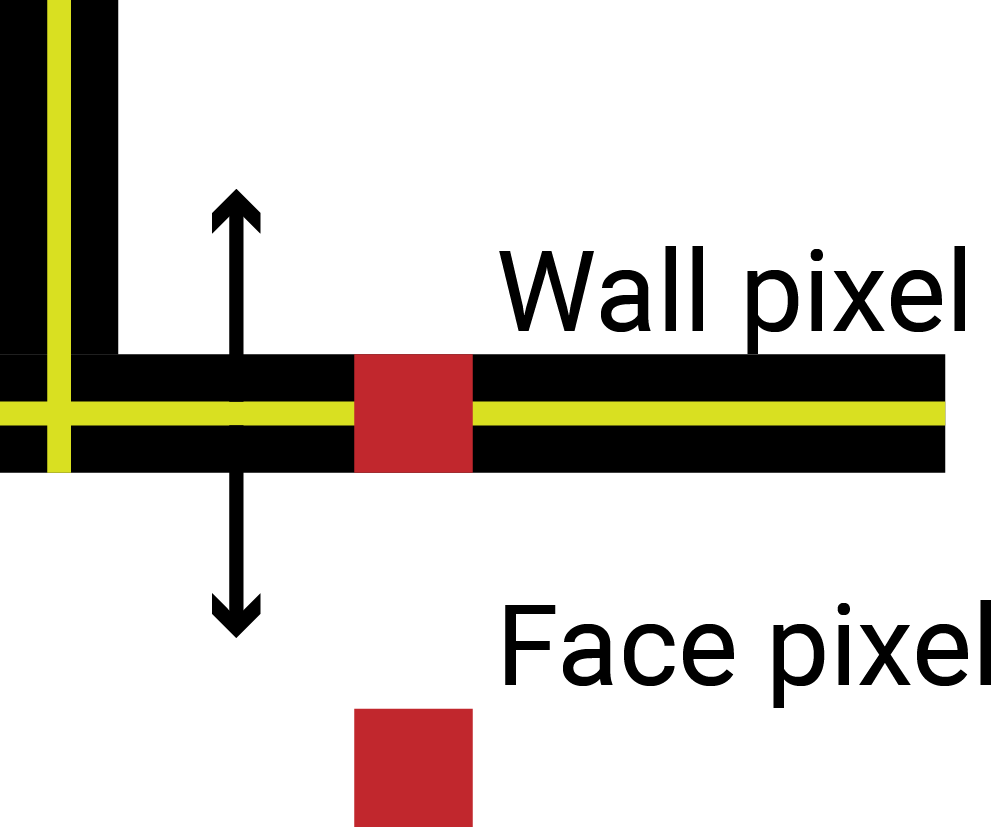
\includegraphics[width=4cm]{images/orientation_computation}
		\caption{Face orientation computation}
		\label{fig:orientation_computation}
	\end{figure}
	
	Because of depth sensor inaccuracy, the computed map pixel coordinate doesn't always lie on the wall. In figure \ref{fig:orientation_computation}, computed face pixel is coloured red. \\ 
	% map pixel coordinate v dictionary
	% "lie on the wall" -> neki drugega v smislu na pixlu, kjer je zid al pa "correspond" namest "lie" - nisem znala zdle pogruntat smiselne zadeve, zato samo komentar.
	
	Using a simple breadth first search in the proximity of the pixel which corresponds to the position of the detected face (from now on \texttt{face pixel}), the closest pixel from the set of pixels, which correspond to the positions occupied by the walls (from now on \texttt{wall pixel}), is determined. In figure \ref{fig:orientation_computation}, this pixel is also coloured red. \\
	% A bi blo bolj smiselno definirat posebi face pixel in wall pixel in ju potem šele uporabit v stavku? (glej prejšnje stanje zgornjega odstavka)
	% Damn it, ne morta bit oba rdeča. Če jih hočemo opisat z barvami, morta bit različnih barv. Sicer ju mormo opisat drugače, recimo dodat oznaki A in B
	
	After the wall pixel has been found, the Hough line finding algorithm is executed on an area around it. The detected lines in figure \ref{fig:orientation_computation} are represented with a yellow colour. If the algorithm finds more than one line, the line which is closest to the wall pixel is selected. After the line is selected, there are two possible orientations as represented in figure \ref{fig:orientation_computation}. The vector that is pointing in the direction of the robot is chosen to be the face orientation. \\ 
	% prestrukturiraj v smislu da normala na najdeno linijo nam določa orientacijo obraza. Ker pa mamo vektorje, sta možni orientaciji dve, vsaka v svoji smeri (v nasprotnih smereh). Ker robot ne vidi skozi zid, pride v poštev tista izmed orientacij, ki je bližje vektorju od pozicije obraza do pozicije robota.
	
	A similar algorithm is used to detect the orientation of the rings (from now on \texttt{ring orientation}).
	% Tuki rabimo še povedat, akj j e pravzaprav orientacija obročka, ker načeloma sam po seb nima orientacije. Mi smo se odločli, da določimo orientacijo kot normalo na ravnino v kateri leži obroček v taki smeri, da lahka robot, ki ima palčko na desni strani (torej robotova desna stran je ob kocki, na kateri je pritrjen obroček), pobere obroček.
	
	\subsubsection{Face classification}
	After faces are detected and localized in the world, they have to be identified.
	
	\subsection{Colour classification} \label{colour_classification}
	The robot must be able to detect the colour of the rings and cylinders. There are six possible classes: black, white, red, green, blue and yellow. \\
	
	In homework 2, we tested different colour spaces and classification models and concluded that the k-nearest neighbours algorithm worked best. The colour space with the highest accuracy in homework was \texttt{HSV} colour model, but in the Gazebo simulator, \texttt{RGB} space worked better. \\
	
	So the colour classifier in the final task uses the k-nearest neighbours algorithm and takes in an input vector in $(red, green, blue)$ format and returns a colour label with one of the six possible classes listed above. \\
	
	Because of the uneven lighting in the Gazebo simulator (and probably in the real world too), the classifier sometimes returns an incorrect label. We solved this problem by using the robustification process as described in the \ref{robustification} section. Colour classifier is run multiple times on different detections of the same object and the most frequent colour is chosen as the colour of the object (from now on \texttt{object colour}). \\
	
	\subsection{Rings}
	In this section, the algorithm for ring detection is presented.
	
	\subsubsection{Ring detection} \label{ring_detection}
	When robot finds the woman that is willing to marry Gargamel, it must help him find a ring that she will like. Luckily, she is kind enough to tell us her favourite colour. The robot must then find the ring in that colour, give it to her and ask her to marry him. \\
	
	But before the ring can be picked up, it must first be detected by the robot. The ring detection is performed on the depth image and the ring colour detection is performed on the \texttt{rgb} image. Again, both images must be synchronized, so it can be accurately localized. \\
	
	% I am not sure that the information below is correct
	Depth image is computed from disparity image, which is calculated from Kinect stereo camera system. The further away an object is, the smaller its disparity will be. Using calibration matrix, depth of each pixel can be approximated from disparity image. Object that appear further away from the camera have a smaller disparity, which reduces the accuracy of depth computation. To combat this, our algorithm first removes all objects that are over a certain distance away from the camera. \\
	
	After inaccurate depths are removed, a blob detection algorithm is applied to our depth image. The algorithm finds regions in our image that differ in colour. It actually searches for dark areas (areas that are further away from the camera) in the depth image. Because the inside of the ring is darker than the ring itself, the inner part is considered a blob. But not all blobs are considered rings. We can then apply some domain knowledge to the problem. We know that all the rings are positioned 12 cm above the cubes, so we can filter all blobs that lie below that height. If we look at the ring from any angle, they look elliptical, so the blobs are filtered by their roundness too. \\
	
	\begin{figure}[h]
		\begin{subfigure}{.5\textwidth}
			\centering
			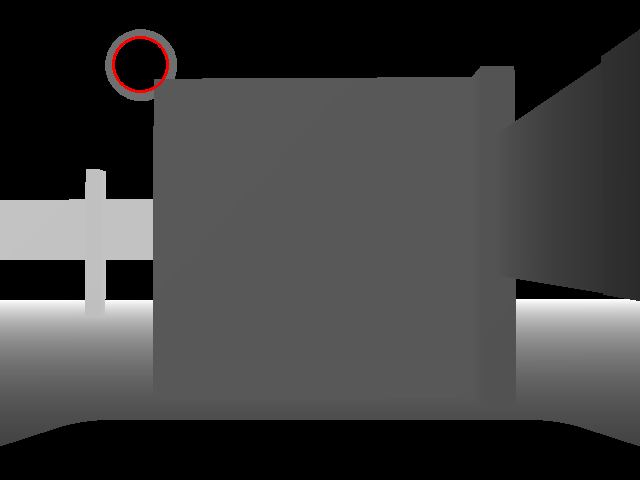
\includegraphics[width=.8\linewidth]{images/ring_detection}
			\caption{Ring detection}
			\label{fig:detected_ring}
		\end{subfigure}%
		\begin{subfigure}{.5\textwidth}
			\centering
			
\includegraphics[width=.8\linewidth]{images/ring_detection_cropped}
			\caption{Cropped ring detection}
			\label{fig:detected_ring_cropped}
		\end{subfigure}
		\caption{Ring detection using blob detector}
		\label{fig:ring_detection}
	\end{figure}

	In figure \ref{fig:detected_ring}, we can see an example of detected ring. Even though the corner of the cube is overlapping with the circle, the ring is still detected. This also presents another problem. To localize the ring, we must know the distance to the ring, but which distance should we use? \\
	
	To compute the distance from camera to the ring, a histogram of distances is created. In figure \ref{fig:distance_histogram}, we can see an example histogram for the figure \ref{fig:detected_ring_cropped} with 24 bins. As we can see, there are two bars that stand out. One of them is the edge of the cube and the other is the ring. A mask is constructed so that only distances that lie in the highest bucket are retained, everything else is removed. \\
	
	\begin{figure}[H]
		\centering
		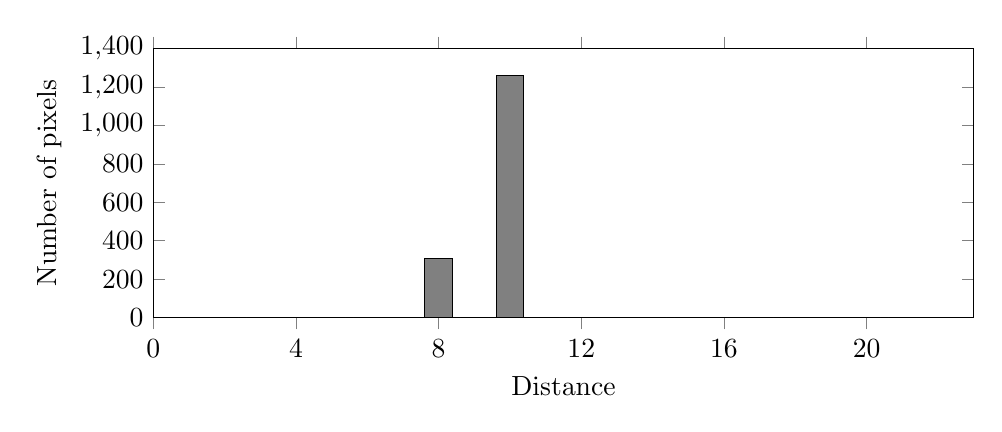
\begin{tikzpicture}
			\begin{axis}[
			ybar,
			xlabel={Distance}, ylabel={Number of pixels},
			xmin=0, xmax=23, ymin=0, ymax=1400,
			xtick={0,4,8,12,16,20,24},
			ytick={0,200,400,600,800,1000,1200,1400,1600},
			width=12cm, height=5cm
			]
			\addplot[fill=gray]
			coordinates {
				(0, 0) (1, 0) (2, 0) (3, 0) (4, 0) (5, 0) (6, 0) (7, 0) (8, 306) (9, 0) (10, 1261) (11, 0) (12, 0) (13, 0) (14, 0) (15, 0) (16, 0) (17, 0) (18, 0) (19, 0) (20, 0) (21, 0) (22, 0) (23, 0) 
			};
			\end{axis}
		\end{tikzpicture}
		\caption{Distance histogram}
		\label{fig:distance_histogram}
	\end{figure}

	The mask is then applied to both, the distance image and the colour image. In figure \ref{fig:masked_colour_ring}, we can see the result of filtering of the \texttt{rgb} colour image using the mask obtained in the previous step. \\

	The distance to the ring is computed as the average of distances to each pixel in the masked distance image. The ring position in world frame is computed using as explained in section \ref{pixel_to_world}. \\

	\subsubsection{Ring colour detection}
	The ring colour is computed using the mask that we have computed in section \ref{ring_detection}. The \texttt{rgb} image is filtered so that only ring is left and then the colour is averaged. The average colour is then classified using the algorithm explained in section \ref{colour_classification}.
	
	\begin{figure}[h]
		\centering
		
\includegraphics[height=5cm]{images/ring_detection_colour}
		\caption{Masked colour ring}
		\label{fig:masked_colour_ring}
	\end{figure}
		
	\subsection{Cylinder detection}
	Cylinder detection runs on a point cloud data that is computed from depth information. \\
	
	\subsubsection{Removal of planes}
	\subsubsection{Cylinder detection}
	
	\subsubsection{Approaching point computation}
	The cylinder approaching point computation is not as difficult as the one for faces. If cylinder has been detected from current robot position, that means that the robot must have a clear view of the cylinder. Because of that, the approaching point can be computed as a point on the line connecting the robot and the cylinder. \\
	
	A point that lies 0.5 metres from the centroid of the cylinder on this line is selected as the approaching point. If the point can't be reached (that is, if it is too close to the wall), approaching point is repositioned so that there is enough space for the robot to visit the point. This is done by finding the closest wall on the map and then moving the point in the opposite direction. This is repeated until there is no wall too close to the point. \\
	
	\subsection{Robustification} \label{robustification}
	The sensors are not 100\% accurate, so we have to take into account some deviation. For example, when an object is detected, the depth sensor might comput the distance inaccurately, or the robot may not have been localized. Detectors might return a false positives and so on. \\
	
	To combat this problem, a robustification is performed on the detected objects. The object detectors send detections to robustifier, which collects data and determines if the detection is a true positive or not. \\
	
	For detection to be considered a true positive, the following must hold true:
	\begin{enumerate}
		\item Detected object was detected at least \texttt{threshold} times
		\item There is at least a \texttt{minimum distance} meters distance between this detection and every other previous detection.
	\end{enumerate}

	If two detections are close enough (the distance between them is less than \texttt{minimum distance}), they are considered the same object. The world position and approaching point position of those two detections are then averaged. So the object position is closer to its actual position in space.
	% world position not defined
	% not ok, zdj se bere kot da nardimo povprečje (detekcija + app.point)/2, kar seveda ni res.
	% Zadnji stavek je treba lepše povezat noter, possibly z vejico, da se priključi prejšnji povedi
	
	\subsection{Smart exploration of space}
	% dobi mapo
	% določi, kje je zid
	% morph
	% delaunayeva triangulacija
	% hierarhical clustering
	% slikici before - after clustering (before naj ma še trikotnike, da se vidi triangualcija - lahka je pa tud posebi slikica sam za trikotnike)
	
	\subsection{Fine movement}
	Fine movement is a special way in which our robot can move. It is used when the normal movement wouldn't be able to get us to the goal even though the goal is reachable.  \\
	% definiraj normal movement

	The \texttt{move\_base} package can be used with \texttt{ROS} to move the mobile base around the map. It uses local and global planner information to avoid obstacles and try to reach the given goal. If it fails to reach the goal, it tries to clear its local map. If that fails, the robot stops trying to reach the goal and notifies us that it has failed to move to the goal. \\
	
	The most common reason for failure is that the goal is too close to any wall in our world. The robot builds a costmap of its environment, where the closer the position is to the wall, the highest cost it has. This way a robot can avoid obstacles and plan the path from point A to point B. The robot builds a costmap in a way that it makes sure not to bump into anything, which means it also takes into account all possible errors in data from its detectors. This means that some of the points that the robot can reach in reality unfortunately fall into the high-cost area and so the normal movement cannot get us there because the risk of bumping into something is too high. \\

	In our final task, the robot had to be able to pick up rings that are positioned very close to the wall. So close actually, that the default movement component is unable to reach the goal. To do that, odometry data must be used and combined with \texttt{Twist} messages to move the robot manually. \\
	
	Because the robot must be able to visit the ring from specific direction (ring orientation), we used a modified version of \texttt{A*} algorithm, that not only finds the shortest path between two points, but also uses the starting and ending robot orientation. \\
	
	Because the world is flat\footnote{Does this make us flat-earthers? Nah. Does this make our robot a flat-earther? Maybe.} and the robot can only rotate along one axis, any robot pose can be represented using a tuple $(x, y, \varphi)$, where $\varphi$ is the orientation along the vertical axis. In theory, the $\varphi$ can be any real number, but in our case, the robot will only have a finite number of possible orientations (the first one being $[0, \frac{2\pi}{n}]$, where $n$ is the number of all orientations). In our final task, we found that $n = 8$ or $n = 16$ works best. \\
	% končno število rotacij zato, da je problem rešljiv. Rešitev se da najt tudi samo z 8 ali 16 različnimi orientacijami. Treba je še dodati, da če imamo 8 možnih rotacij, mora A* kr naenkrat preiskat 8*height*width pixlov (trojic x,y,fi) in že to kr poveča kompleksnost.
	% n=8 pomeni 45-stopinjske obrate

	% dodaj slikico možnih orientacij
	\begin{figure}[h]
		\centering
		\vspace{6cm}
		\caption{All possible orientations a robot can have if n=8 (blue/left) and if n=16 (red/right)}
		\label{fig:possible_orientations}
	\end{figure}

	The algorithm will use map to access environment information, so the $x$ and $y$ represent pixel coordinate in map coordinate system.
	% razloži kaj dejansko pomenijo te (x, y) koordinate pod imenom pixli. V kaki relaciji so z globalnimi koordinatami/posi od robota?
	
	% Image of the robot and the next three possible states
	\begin{figure}[h]
		\centering
		\vspace{6cm}
		% 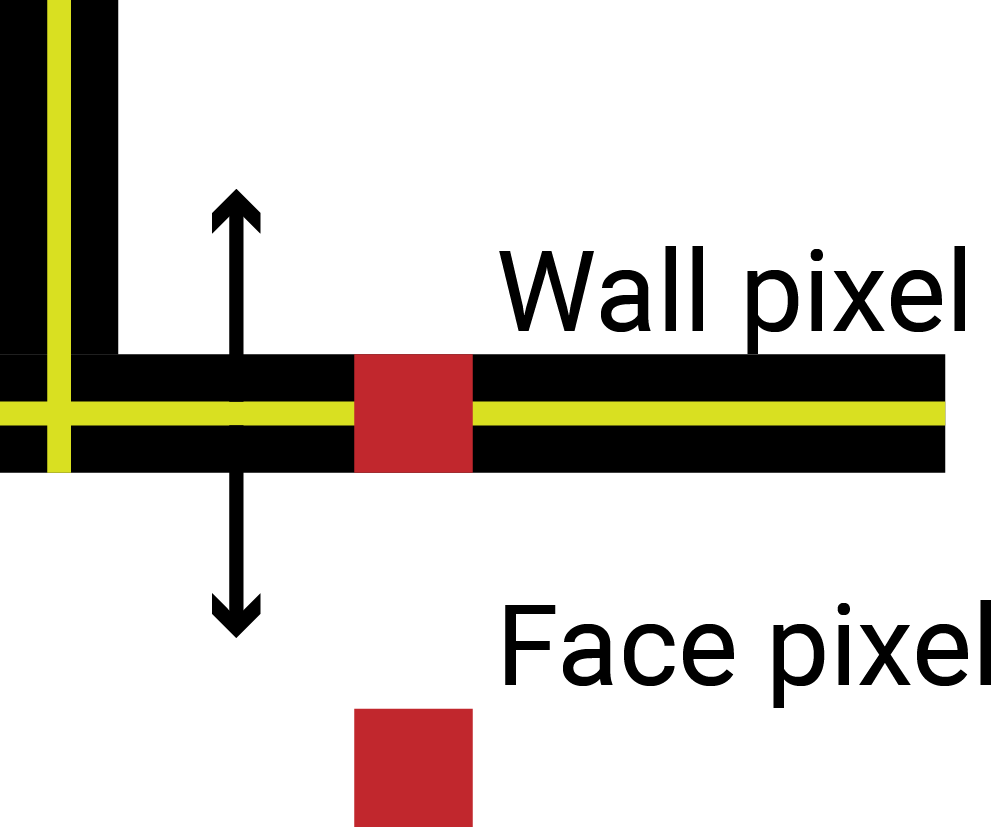
\includegraphics[width=4cm]{images/orientation_computation}
		\caption{Next possible robot states}
		\label{fig:next_robot_states}
	\end{figure}
	
	If the robot is currently in state $\vec{s_i} = (x_i, y_i, \varphi_i)$, we can define the next states to be:
	
	\begin{enumerate}
		\item Move forward
		$$\vec{s_{i+1}} = (x_i + \alpha \cos \varphi_i, y_i + \alpha \sin \varphi_i, \varphi_i)$$
		\item Rotate left by $\frac{2\pi}{n}$ and move forward
		$$\vec{s_{i+1}} = (x_i + \alpha \cos \varphi_i, y_i + \alpha \sin \varphi_i, \varphi_i - \frac{2\pi}{n})$$
		\item Rotate right by $\frac{2\pi}{n}$ and move forward
		$$\vec{s_{i+1}} = (x_i + \alpha \cos \varphi_i, y_i + \alpha \sin \varphi_i, \varphi_i + \frac{2\pi}{n})$$
	\end{enumerate}
	
	Where $\alpha$ is the step size (to move 1 pixel forward, $\alpha = 1.5$). Each state is only possible if the map does not contain a wall at pixel $(x_{i+1}, y_{i+1})$. Because the orientations are cyclical, if the robot orientation is less than $0$ or more than $2\pi$, the orientation is wrapped around to be inside $[0, 2\pi]$ range. \\
	% zakaj je alfa 1,5: dodaj slikico al pa razloži, da zato, ker če je 1, lahka gremo sam gor dol levo desno, ne pa tud diagonalno.
	% "Each state" ali "Each step"?
	% "not contain a wall at pixel $(x_{i+1}, y_{i+1})$" dodaj, da je to pixel, na kerga se želimo prestavit/na kerga nas pripelje korak
	
	The heuristic function can be defined as an Euclidean distance between current state and the end state. $$h(s_i) = \sqrt{(x_{end} - x_i)^2 + (y_{end} - y_i)^2 + (\varphi_{end} - \varphi_i)^2}$$. To avoid getting too close to the walls, a penalty is added to the pixels that are too close to the wall. \\
	
	The \texttt{A*} algorithm can now be run using states as defined above. We start with initial robot state $(x_0, y_0, \varphi_0)$ and set the goal to the ring position $(x_m, y_m, \varphi_m)$. The closest path between those two states is the path that the robot should follow to get from its current position to the goal position including its orientations. \\
	
	After the path is computed, the robot can subscribe to odometry data to get its position and follow the list of poses that the previous algorithm has computed. To move from one pose to another, we wait until next odometry message is received, then rotate until we are oriented in the direction to the next goal and then move until we are close enough to the next pose. \\
	
	\section{Implementation and integration}
	In this section, the implementation of the algorithms explained in section \ref{methods} will be discussed. To solve our task, the following architecture was designed. We tried to keep the entire project as modular as possible, not only because this is the \texttt{ROS} operating system's philosophy, but also because three different people needed to work on the same project at the same time. \\ % tale zadnji stavek bi se dalo še mal boljš ubesedit
	
	This proved to be very difficult because nodes are so interconnected, that if any part of the system didn't work as intended, it seemed as if nothing worked. Some parts of the system were discussed beforehand, but as the tasks became more difficult, the arhitecture had to be changed in order to solve them. \\ 
	
	\begin{figure}[h]
		\centering
		\caption{Final architecture}
		\label{fig:final_architecture}
	\end{figure}
	
	\subsection{Object detectors}
	There are three different nodes responsible for object detections. Face and ring detectors are using \texttt{rgb} and depth images and the cylinder detector is using point cloud and \texttt{rgb} image to detect object in our world. \\
	
	All three object detectors are publishing a custom \texttt{ObjectDetection} message type. The \texttt{Robustifier} component subscribes to this type of message and tries to minimize the number of false positives. 
	
	\subsubsection{ObjectDetection message}
	The object detection message contains the following information
	\begin{enumerate}
		\item \texttt{Header header}, which contains the timestamp of the detection and other metadata
		\item \texttt{string type}, which represents the type of the detected object (it can be either \texttt{"face"}, \texttt{"ring"} or \texttt{"cylinder"})
		\item \texttt{Pose object\_pose}, which represents the object position in world coordinate frame
		\item \texttt{Pose approaching\_point\_pose}, which is a point that the robot has to visit in order to complete the task
		\item \texttt{Image image}, which is an image of the object
		\item \texttt{ColorRGBA color} color and \texttt{string classified\_color} which represent the object average colour in \texttt{RGBA} format and the colour label that the colour classifier computed
	\end{enumerate}

	% Why have we decided that we needed object detection message. Because of our robustification process.
	
	\subsubsection{Face detector node}
	The face detector is responsible for detecting and localizing faces. To do that, it fist synchronizes received \texttt{rgb} and depth images using the \texttt{Time Synchronizer} class in \texttt{message\_filters} package. \\

	After both, the \texttt{rgb} and depth images are received, it uses the Haar cascade algorithm explained in section \ref{face_detection_algorithm} to detect faces. If face has been found, it tries to compute its world position. This is done using raycasting from camera center, through the face center pixel in the image plane as explained in section \ref{pixel_to_world}. \\

	After face is localized, \texttt{Approaching point} is computed. \texttt{Approaching point} is a point that is positioned directly in front of the face. Because the faces are positioned on the walls, the closest wall to the face is found. Then, the wall normal is computed as explained in section \ref{face_orientation_computation}. The \texttt{Approaching point} is positioned 0.5 metres from the face position in the direction of the face orientation. \\

	\subsubsection{Ring detector node}
	Ring detector is a node that is responsible for ring detection and localization. It works similarly to the face detector node. First, it synchronizes depth and \texttt{rgb} images. Then it uses the ring detection algorithm as explained in section \ref{ring_detection}. Ring localization is done using the algorithm explained in section \ref{pixel_to_world}. \\
	
	Ring orientation is determined using similar algorithm as explained in section \ref{face_orientation_computation}, but instead of finding the normal of the wall, its direction is chosen as ring orientation. \\ % tu bi blo mogoč boljše vseen še enkrat povzet, kk deluje, ker če ne more bralec it pogledat nazaj gor, kje zamenjamo to normalo
	
	\subsubsection{Cylinder detector node}

	\subsection{Robustifier}
	For each object detector, a new \texttt{Robustifier} node is created. So each \texttt{Robustifier} node is listening for different object detections. The detections are then grouped together using the algorithm as explained in section \ref{robustification}. When number of detections sent to the \texttt{Robustifier} node exceeds the \texttt{threshold} value, the detection is considered a true positive and is sent to the \texttt{Brain} node. \\
	
	\subsection{Brain}
	\texttt{Brain} is a node that is responsible for solving the main part of the task. It subscribes to robustified object detections and uses them to solve the task. \\
	% Main part of the task?
	
	% Manjka, ker se ne vemo kako bo delalo
	
	\subsection{Movement controller}
	
	\subsection{Greeter}
	
	\section{Results}
	\section{Division of work}
	% We should only write what each of us did here and add that the professor should compute percentages himself.
	
	\section{Conclusion}	
	
\end{document}